% !TEX program = xelatex
%Wzór dokumentu
%tu zmień marginesy i rozmiar czcionki
\documentclass[a4paper,12pt]{article}
\usepackage{inputenc}[utf8]
\usepackage[margin=2.5cm]{geometry}

%Lepiej tego nie zmieniaj, jak co to dodawaj pakiety
\usepackage{titlesec}
\usepackage{titling}
\usepackage{fancyhdr}
\usepackage{mdframed}
\usepackage{graphicx}
\usepackage{amsmath}
\usepackage{amsfonts}
\usepackage{multicol}
\usepackage{listings}
\usepackage{caption}
\usepackage{float}

\captionsetup[figure]{name=Załącznik}
\captionsetup[table]{name=Tabelka}

%inny wygląd
%\usepackage{tgbonum}


%Zmienne, zmień je!
\graphicspath{ {./ilustracje/} }
\title{bfc64 - dokumentacja}
\author{Grzegorz Koperwas}
\date{\today}

%lokalizacja polska (odkomentuj jak piszesz po polsku)

\usepackage{polski}
\usepackage[polish]{babel} 
\usepackage{indentfirst}
\usepackage{icomma} 

\brokenpenalty=1000
\clubpenalty=1000
\widowpenalty=1000    

%nie odkometowuj wszystkiego, użyj mózgu
%\renewcommand\thechapter{\arabic{chapter}.}
\renewcommand\thesection{\arabic{section}.}
\renewcommand\thesubsection{\arabic{section}.\arabic{subsection}.}
\renewcommand\thesubsubsection{\arabic{subsubsection}.}

%Makra

\newcommand{\obrazek}[2]{
\begin{figure}[h]]
    \centering
    \includegraphics[scale=#1]{#2}
\end{figure}
}     
        

\newcommand{\twierdzonko}[1]{
    \begin{center}
    \begin{mdframed}
    #1
    \end{mdframed}          
    \end{center}
} 

\newcommand{\dwanajeden}[2]{
\ensuremath \left( \begin{array}{c}
    #1\\
    #2
\end{array} \right)
}  

%Stopka i head (sekcja której nie powinno się zmieniać)
\pagestyle{fancy}
\fancyhead{}
\fancyfoot{}

%Zmieniaj od tego miejsca
\rfoot{\thepage}
\lfoot{Grzegorz Koperwas}
\lhead{}
\rhead{Ostatnia edycja: \today}
\renewcommand{\headrulewidth}{1pt}
\renewcommand{\footrulewidth}{1pt}

\begin{document}
    \begin{titlepage}
    Politechnika Śląska

    Wydział Matematyki Stosowanej

    Kierunek Informatyka

    \begin{center}
        Gliwice, \today

        \vspace{2cm}

        \Large{Programowanie I}

        \vspace{5mm}

        \Large{\bfseries{Projekt zaliczeniowy}}

        \vspace{5mm}

        \large{,,BFC64''}

        \vspace{2cm}

        \theauthor{} gr. 2 lab 2C
	\end{center}
	\thispagestyle{empty}
    \end{titlepage}
    \tableofcontents
    \section{Opis projektu}

    Projekt jest kompilatorem języka \emph{brainfuck},\footnote{Nie zawierającym linkera oraz assemblera.Patrz sekcja \ref{usecase}} 8 bitowym, nie pozwalającym na overflow'y\footnote{Typ non-wrapping}. Powinno się dać go łatwo portować na inne systemy oparte o procesor \texttt{MOS 6502/6510}, czy inne architektury.

    \section{Wymagania}

    \begin{itemize}
        \item Kompilacja do assemblera kickassembler
        \item Ośmiobitowa ,,taśma'' o długości większej niż 256 bajtów, w formie \emph{non-wrapping}
        \item Optymailzowanie kodu w postaci \texttt{++++++--+} na pojedyńcze symbole
    \end{itemize}

    \subsection*{Wymagania ,,poza konkursem''}

    \begin{itemize}
        \item Możliwość łatwej rozbudowy o inne architektury.
        \item Stworzenie kompilatora, a nie interpretera w assemblerze, kosztem pamięciożerności.
        \item Nauka assemblera.
        \item Kod który da się łatwo edytować, z tego powodu plik \texttt{template.cpp} jest generowany skryptem pythona by nie musieć go pisać ręcznie. W innym wypadku musiał bym ręcznie zmieniać kod podobny do tego w załączniku \ref{crazycpp}.
    \end{itemize}

    \begin{figure}[h]
        \begin{lstlisting}[language=c,frame=L,basicstyle=\footnotesize\ttfamily]
std::string
subtract(std::string value, std::string label, std::string label2)
    {
        return "    lda ($fb),y\n    clc\n    cmp #" + value
               + "\n    bcs " + label + " //if lower than "
               + "number\n    lda #$00\n    jmp " + label2
               + "\n" + label + ":\n    sec\n    sbc #" + value
               + "\n" + label2 + ":\n    sta ($fb),y\n";
    }
        \end{lstlisting}
        \caption{Nie, nie piszę tego.}
        \label{crazycpp}
    \end{figure}

    \section{Przebieg realizacji}

    Sama implementacja podstawowej logiki kompilatora nie sprawiła większych problemów, toż to nie będę się rozpisywał na jej temat. Parserem jest zwykłą pętlą, podobnie jest z optymalizatorem.

    Największe trudności sprawiało zaimplementowanie taśmy o długości większej niż 256 komórek. Okazuje się że koncept pointerów, ze względu na 8 bitowość procesora posiadającego 16 bitową szynę adresową, jest wykonywany przez ten procesor \emph{ciekawie...}

    Łącząc to z pierwszymi próbami używającymi rejestru \texttt{X} procesora zamiast \texttt{Y}, zamiast wartości na taśmie programy zmieniały wartość pointera. Dodając to iż procesor jeszcze ładnie indeksował pointer rejestrem \texttt{X} to programy dla paru komórek taśmy działały, potem dziwiłem się czemu taśma nie jest zerowa. Spowodowane to było tym iż właśnie okolica adresu który wybrałem na lokalizację pointera była nie używana przez Kernal, jednak obok były już nie-zerowe rejestry systemowe oraz basic'a.

    Po dniu debugowania programem \texttt{C64-Debugger}\footnote{https://sourceforge.net/projects/c64-debugger/}, którego obsługa jest ciekawa. Sam interfejs (patrz rysunek \ref{c64-debug}) nie daje żadnej wskazówki jak z niego korzystać, ale po zrozumieniu breakpointów udało się go opanować.

    \begin{figure}[h]
        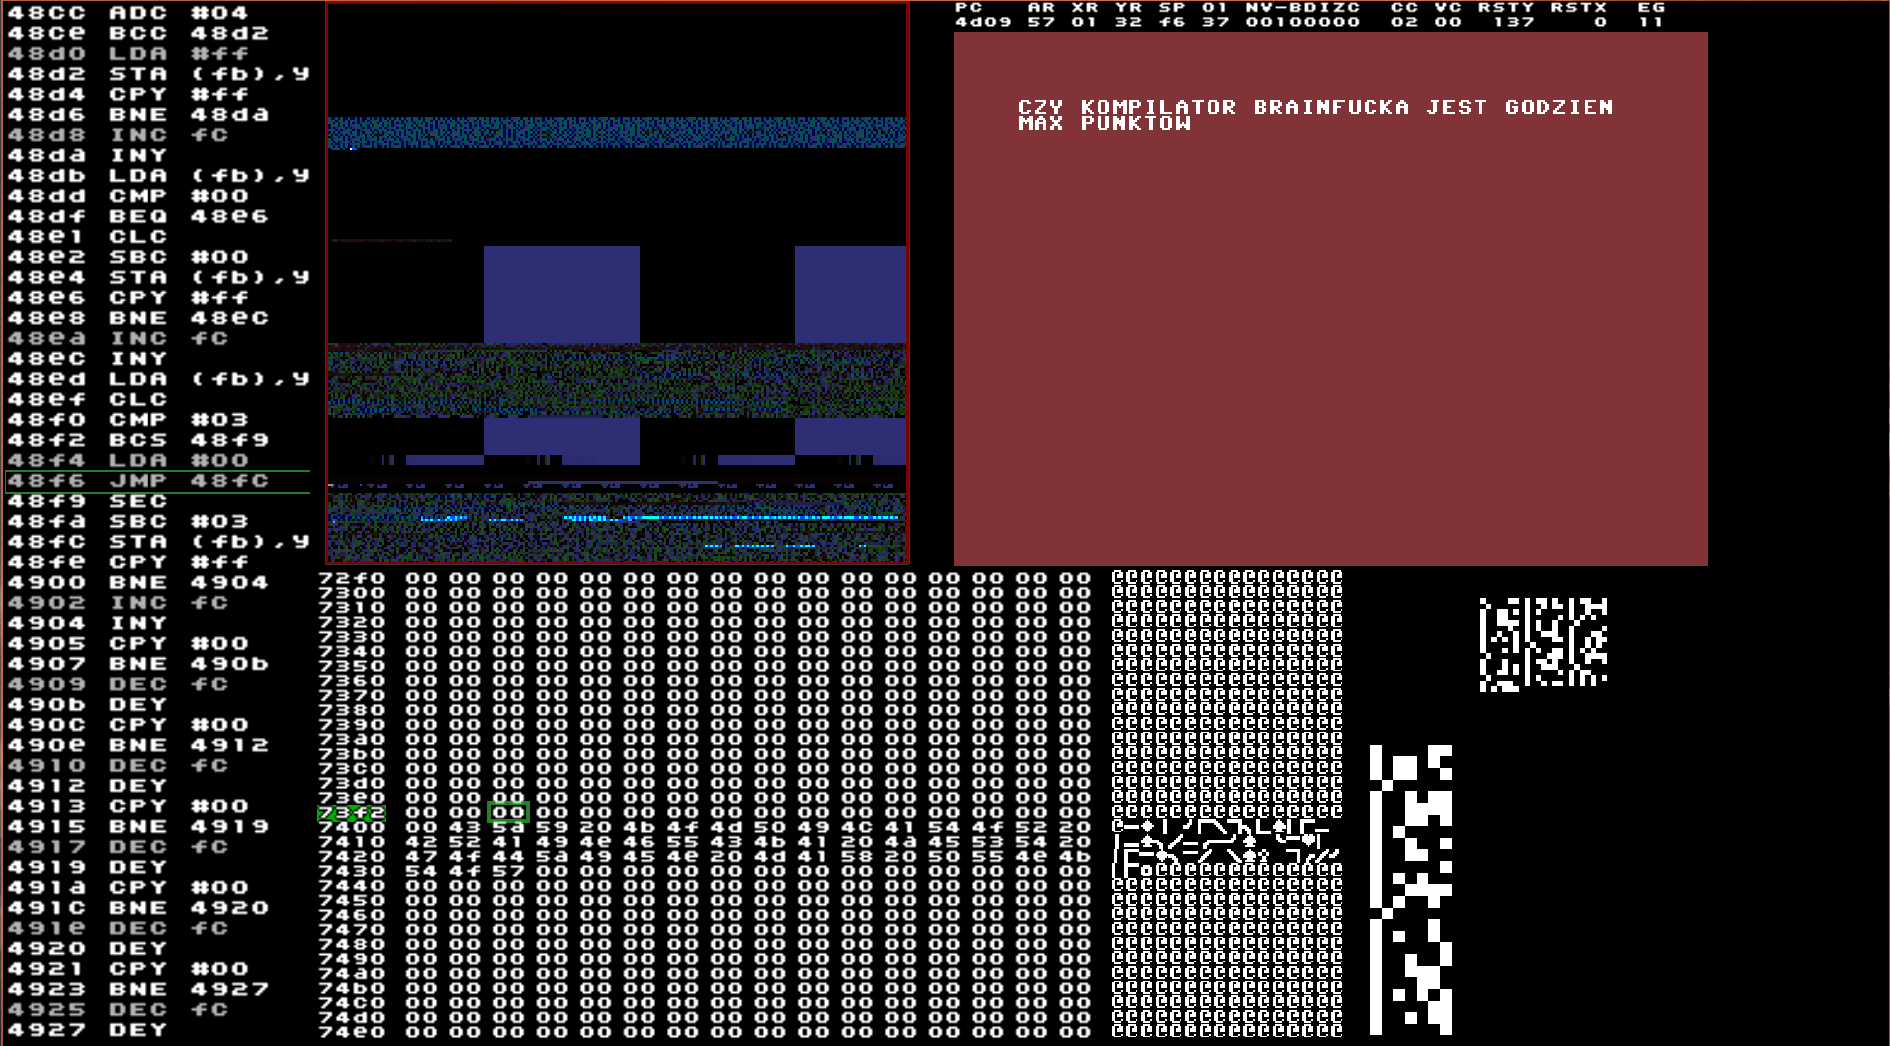
\includegraphics[scale=0.3]{c64debug.png}
        \centering
        \caption{\emph{Interfejs} programu \texttt{C64-debugger}, $\frac{10}{10}$ would debug again}
        \label{c64-debug}
    \end{figure}

    Dodatkowe szczegóły na temat pracy programów po kompilacji znajdują się w sekcji \ref{wzorce}

    \section{Instrukcja użytkownika i opis działania}

    \subsection{Kompilowanie}

    \subsubsection*{Wymagania do kompilacji:}
    \begin{itemize}
        \item gcc - kompilator
        \item make
        \item python - generowanie pliku \texttt{template.cpp} (patrz kompilator)
        \item xelatex - dokumentacja
    \end{itemize}

    Kompilujemy poleceniem \texttt{make}.

    \vspace{5mm}

    Instalujemy poleceniem \texttt{sudo make install}

    \vspace{5mm}

    Dokumentacje kompilujemy poleceniem \texttt{make docs}.

    \vspace{5mm}

    Przykładowy test uruchamiamy poleceniem \texttt{make test}, powinien uruchomić emulator Vice z programem testowym \texttt{tests/test.b}.

    \subsubsection*{Wymagania do używania}\label{usecase}

    \begin{itemize}
        \item kickassembler\footnote{http://theweb.dk/KickAssembler/Main.html\#frontpage} - bfc64 generuje pliki \texttt{.asm} dla tego assemblera
        \item System Linux, testowane wyłącznie na Arch'u
    \end{itemize}

    Program uruchamiamy poleceniem \texttt{bfc64 <ścieżka do pliku źródłowego>}, utworzy on plik a.asm gotowy do przetworzenia kickassemblerem za pomocą polecenia \texttt{kickass a.asm}. Utworzy on nam plik wykonywalny \texttt{a.prg} dla commodore 64 lub emulatora.

    Emulator Vice\footnote{https://vice-emu.sourceforge.io/} uruchomi automatycznie programy poleceniem:
    \begin{lstlisting}[frame=single,basicstyle=\ttfamily]
$ x64sc -autostart $PWD/a.prg
    \end{lstlisting}

    \subsection{Działanie kompilatora bfc64}

    Kompilator składa się z trzech głównych części:
    \begin{itemize}
        \item Parsera - zamieniającego pliki tekstowe na listę symboli
        \item Optymalizatora zamieniającego sąsiednie \texttt{++++--} na operacje dodawania lub odejmowania.
        \item Kompilatora - zamieniającego listę symboli na kod assemblera korzystając z funkcji z przestrzeni \texttt{arch}
    \end{itemize}

    \subsubsection*{Parser}

    Parser jest funkcją \texttt{parseSourceFile}, która przyjmuje jako argument plik z kodem źródłowym. Zamienia ona wewnętrznie znaki języka \emph{brainfuck} na odpowiadające im symbole według tabelki \ref{tab:symbole}.

    \begin{table}[H]
        \begin{tabular}{|c|l|}
            \hline
            Symbol         & Wartość   \\ \hline
            +              & inc       \\ \hline
            -              & dec       \\ \hline
            \textless{}    & left      \\ \hline
            \textgreater{} & right     \\ \hline
            {[}            & loopBegin \\ \hline
            {]}            & loopEnd   \\ \hline
            ,              & in        \\ \hline
            .              & out       \\ \hline
        \end{tabular}
        \centering
        \caption{Symbole oraz odpowiadające im wartości z \texttt{SymbolType}}
        \label{tab:symbole}
    \end{table}

    Dodatkowo parser wyświetla ostrzeżenia w przypadku jeśli w trakcie pętli za każdą iteracją jest porównywalna inna komórka pamięci, na przykład dla pętli \texttt{[>><]} zostanie wyświetlone ostrzeżenie wraz z numerem lini początkowym i końcowym.

    Jeśli parser napotka \texttt{]} bez poprzedniego \texttt{[} czy nie znajdzie w pliku końca pętli przed jego końcem zgłosi on błąd użytkownikowi i nie skompiluje programu.

    Parser traktuje wszystkie inne znaki jako komentarz.
    
    \subsubsection*{Optymalizator}

    W celu ograniczenia pamięci potrzebnej na załadowanie programu optymalizator zamienia sąsiednie symbole \texttt{+} oraz \texttt{-} na symbole specjalne \texttt{add} oraz \texttt{subtract}. W planach jest dodanie zamieniania \texttt{>} i \texttt{<} na symbole specjalne \texttt{jmpLeft} oraz \texttt{jmpRight}

    \subsubsection*{Kompilator}

    Kompilator tworzy stringa na podstawie listy symboli z parsera za pomocą wzorców generowanych podczas kompilacji z plików w folderze \texttt{processor/arch/c64}. Dodatkowo na początek dołącza \texttt{arch::begin} a na koniec \texttt{arch::end}

    Wzorce, z których korzysta kompilator są generowane automatycznie skryptem pythona \texttt{templateGen.py}. Generuje on plik źródłowy \texttt{template.cpp} z pomocą pliku-wzorca \texttt{template.cpp.template}, do którego podstawia za placeholdery\footnote{W formie \texttt{\$nazwa}} odpowiednie sumy stringów oraz parametrów funkcji według plików-wzorców assemblera, w których podmienia \texttt{label()} na argument \texttt{label} itd. Opis wzorców w sekcji \ref{wzorce}.


    Wygenerowany \texttt{string} program zapisuje do pliku wyjściowego.

    \subsection{Opis działania skompilowanego programu}\label{wzorce}
    
    \subsubsection*{Wyzwania architektury 6502/6510/commodore 64}

    Procesory \emph{MOS 6502/6510} posiadają 8 bitową szynę danych oraz 16 bitową szynę adresową. Z tego powodu ,,pointery'' muszą się znajdować w pierwszych 256 bajtach pamięci, tak zwanej ,,zeropage''. Kompilator umieszcza w pamięci o adresie \texttt{\$00FB} adres \texttt{\$7300}, który jest adresem początku taśmy. 

    Procesor posiada opcje indeksowania pamięci rejestrem Y, taki odpowiednik $\left(\texttt{pointer} + \texttt{rejestr}_Y \right)^*$ w języku \texttt{C++}. Jednak jako iż rejestr \texttt{Y} jest 8 bitowy, a chcemy taśmę o długości większej od 256 to ruch po taśmie w lewo wygląda tak:

    \begin{figure}[H]
        $\vdots$
    \centering
        \vspace{-3mm}
        \begin{lstlisting}[basicstyle=\ttfamily,morekeywords={cpy,bne,dec,dey}]
                cpy #$00      // compare Y to 0
                bne label()   // if Y != 0 goto label
                dec $00fb + 1 // decrement tape pointer
            label():
                dey           // decrement Y
        \end{lstlisting}
        \vspace{-3mm}
        \centering
        $\vdots$
    \centering
    \end{figure}

    \subsubsection*{Taśma}

    Definicja taśmy, w pliku \texttt{end.asm}, wygląda tak:

    \begin{figure}[H]
        \begin{lstlisting}[basicstyle=\ttfamily,morekeywords={cpy,bne,dec,dey,fill}]
            *=$7300 "Tape"    // at address $C000
                .fill 1024, 0 // place 1024 zeros
        \end{lstlisting}
    \end{figure}

    Generuje ona taśmę o długości 1024 bajtów, jednak jako iż kompilator nie zabezpiecza nas przed ,,wyjściem'' z jej przestrzeni, zatem jeśli komuś chce się pisać dużo \texttt{>} i wiedząc iż adres pierwszej komórki to \texttt{\$73FF}/\footnote{Początek taśmy \texttt{\$7300} + początkowa wartość \texttt{Y} równa \texttt{\$ff}} możemy zmieniać kolory tła, tekstu, odtwarzać muzykę oraz nadpisywać program.

    \subsubsection*{Wypisywanie znaków na ekran i ich odczyt}

    Kernal commodore 64 posiada \emph{funkcje}, które realizują te zadania.

    Pod adresem \texttt{\$FFCF} jest funkcja, która umieszcza w rejestrze A wartość wprowadzoną przez użytkownika.

    Pod adresem \texttt{\$FFD2} jest funkcja, która wartość w rejestrze A wypisuje na ekran.

    Wadą tych funkcji jest to iż nie używają zestawu znaków ASCII, tylko własnego PETSCII\footnote{https://www.c64-wiki.com/wiki/PETSCII}. Z tego powodu przy wypisywaniu na ekran za pomocą ,,\texttt{.}'' trzeba ustawiać wartość komórki na wartości PETSCIII.

    \subsubsection*{Wzorce}

    Kompilator korzysta z wzorców w folderze \texttt{processor/arch/c64}, które są plikami assemblera które są wstawiane za odpowiednie symbole. Za symbol \texttt{inc} wstawia \texttt{inc.asm} itd. Są one przetwarzane przez skrypt pythona do pliku \texttt{template.cpp} podczas kompilacji by nie było potrzeby wpisywania ich na sztywno.
    
    Przykładowo w załączniku \ref{kod:inc} do rejestru \texttt{A} ładowana jest wartość aktualnej komórki, następnie porównywana jest z \texttt{\#\$ff}\footnote{\# oznacza że jest to wartość a nie adres}. Jeśli zachodzi równość, program przechodzi do \texttt{label}, w innym przypadku upewnia się że flaga \texttt{carry} jest wyłączona i dodaje do rejestru \texttt{A} jedynkę. Następnie zapisuje wynik w pamięci.

    \begin{figure}[h]
        $\vdots$
        \centering
        \vspace{-3mm}
        \begin{lstlisting}[basicstyle=\ttfamily,morekeywords={cpy,bne,dec,dey}]
                            lda ($fb),y
                            cmp #$ff
                            beq label()
                            clc
                            adc #$01
                            sta ($fb),y
                        label():
        \end{lstlisting}
        \vspace{-3mm}
        $\vdots$
        \centering
        \caption{Zwiększanie komórki o 1}
        \label{kod:inc}
    \end{figure}
    \end{document}
